\documentclass[12pt]{article} 

\usepackage[utf8]{inputenc} % set input encoding (not needed with XeLaTeX)

\usepackage[bottom = 1.5in]{geometry} % to change the page dimensions
\geometry{a4paper} % or letterpaper (US) or a5paper or....
% \geometry{margin=2in} % for example, change the margins to 2 inches all round
% \geometry{landscape} % set up the page for landscape
%   read geometry.pdf for detailed page layout information
%%% PAGE  SETUP

\usepackage{fancyhdr}

\pagestyle{fancy}
\lhead{Joshua Redona}
\rhead{\thepage}
\cfoot{} %gets rid of numbers


%%% PAGE SETUP DONE
\usepackage{amsmath}
\usepackage{amssymb}
\usepackage{forest}
\usepackage{tikz}
\usetikzlibrary{datavisualization}
\usetikzlibrary{datavisualization.formats.functions}

\usepackage{graphicx}
\graphicspath{ {./assets/} }

\DeclareSymbolFont{symbolsC}{U}{txsyc}{m}{n}

% ---- \begingroup
\title{Intro to AI}
\author{Joshua Redona, David Harianto}
%\date{} % Activate to display a given date or no date (if empty),
         % otherwise the current date is printed 

\begin{document}
\maketitle
% ---- \endgroup

\section*{Bot 4 Design}
Our Bot 4 algorithm is quite simple, and combines aspects of Bots 1 and 2. During each step, 
the bot will check whether or not any of the routed cells are on fire, and will replan 
only when it sees one of these cells has fire spread. The only information it accounts for 
is if its current path is still viable, and if it is not it will try to make a new path to follow.

\section*{Success Graph for Various Values of q}
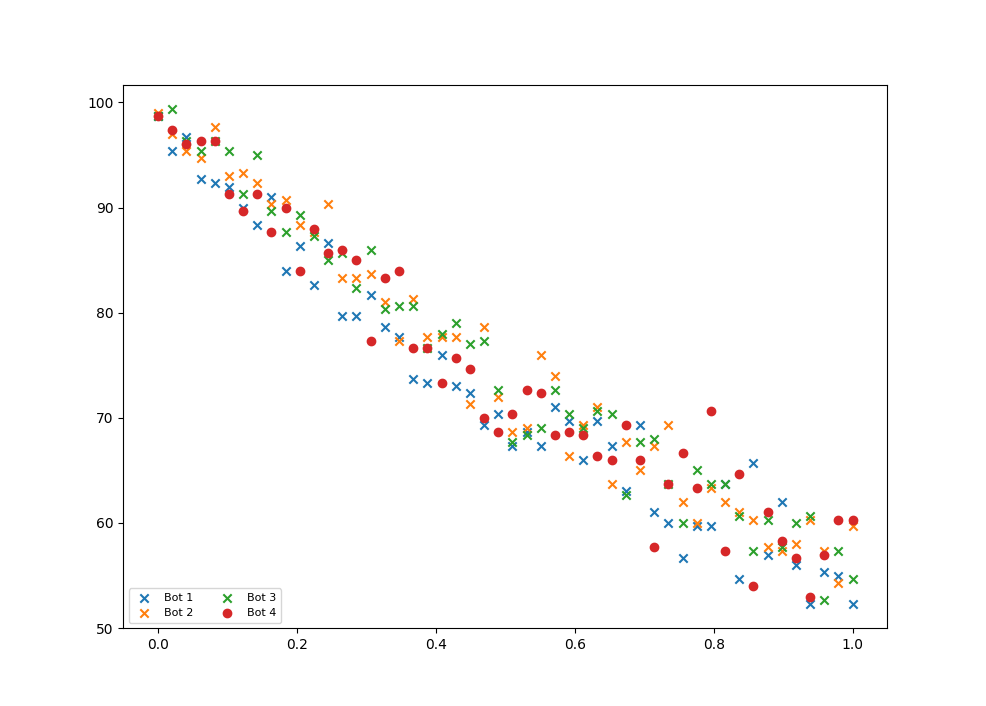
\includegraphics[scale=0.61]{Figure_3}
\\
Included is the graph of each bot's success rates (out of 100 \text{\%}) plotted against 
the value of q used. For the graph above, we used values ranging from 0 to 1 with a step size of 
0.02 between. For each bot and q value, 300 simulations of the ship were performed in order to get an 
accurate measure of success.  

\section*{Why do our bots fail?}
Surprisingly, many of the bot failures result from a poor starting position. Especially for bots 2 and 3, many of the
graph failures that are printed appear after only a few steps and occur when the button is completely covered by fire,
(meaning no possible path exists to plan). We expected to have bots that fail because they take the shortest path 
and do not try to plan a path that is far from the fire, but more times than not there is only one open adjacent square 
to the button, and when it is burned the bot fails no matter where on the board it is. 
\\
\\
It is worth noting that for q=0, the only failures come from bot 1 if it gets unlucky, or from a starting position that is impossible. 
For q=0.5, once again many of our failures come from the only path to the button being burned away. In one specific case for
Bot 4 at q=0.5, a failure occurred because the bot went down a narrow path of squares with its only exit being blocked by fire. In this sense, 
we learned that an ideal bot would try to avoid narrow parts of the graph in order to avoid failing by being blocked in. 
\section*{Ideal Bot Construction}
An ideal bot would take into account the probability of fire spreading in order to better plan its routes 
to the button. It would also be able to distinguish squares that would trap itself with fire (say 
enclosed rows and columns that require backtracking) and immediately avoid planning over those squares. 
\\
\\
Something that we discussed (but decided was not feasible to implement) was to have a bot make decisions for a q=1 board where fire spread 
was guaranteed and make decisions based off that. Similar to bot 3, this bot would avoid adjacent fire squares, but also account for paths 
that would be closed off from the fire before the bot could get there. Of course, if any of the fire spread, this bot would still make 
the optimal move for that turn, and if the fire did not spread we could resimulate the q=1 board for the new position. 

\end{document}
